Для сборки проекта был выбран Webpack из-за удобной работы с одностраничными приложениями, продвинутого разделения кода и Hot Reload для более быстрой разработки с помощью React.
Webpack -- система сборки, которая предоставляет не только бандлинг (компоновку) модулей, но и может выполнять задачи, которыми занимаются Gulp/Grunt. К тому же, Webpack не 
ограничивается JavaScript-файлами, он может работать с другой статикой вроде CSS, картинок, html-компонентов и др. Webpack также поддерживает очень полезную фичу -- code splitting 
(разбиение кода). Большое приложение можно разбить на куски, которые загружаются по мере необходимости.

Бандлеры позволяют упаковывать, компилировать, организовывать множество ресурсов и библиотек, необходимых для современного веб-проекта.

\begin{figure}[ht]
\centering
  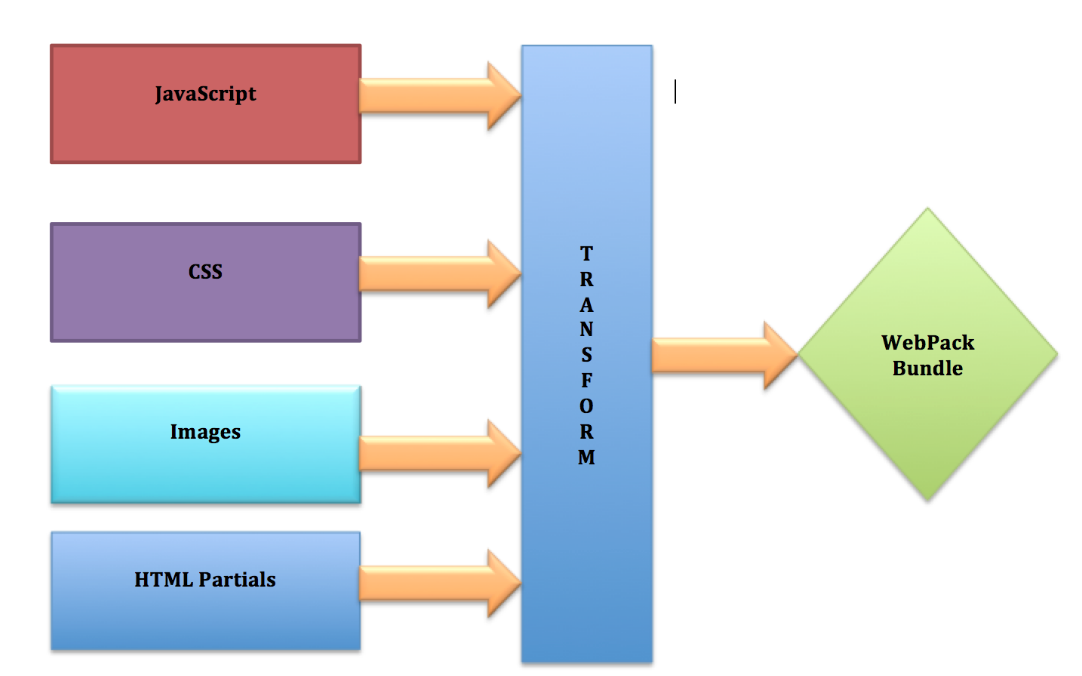
\includegraphics[scale=0.40]{webpack.png}
  \caption{Схема процесса сборки webpack}
  \label{figure:domain:webpack}
\end{figure}

Webpack:
\begin{itemize}
\item автоматически строит дерево зависимостей ресурсов.
\item упаковывает модули, которые могут быть загружены «лениво», в отдельные файлы.
\item выполняет оптимизацию кода.
\item может делать «горячую» замену модулей на странице.
\end{itemize}

Начало работы с WebPack 

Как и большинству инструментов Web-разработчика, Webpack требует для своей работы установленный Node.js. Если Node.js уже настроен, то все, что нужно с
делать для установки Webpack -- это выполнить следующую команду в консоли:
\begin{lstlisting}[language=bash, label=lst:domain:html]
npm install webpack --g
\end{lstlisting}

Данная команда установит Webpack глобально в системе, что позволит запускать его из любого места. Далее, внутри директории проекта, был создан
файл index.html с начальной разметкой:
\begin{lstlisting}[language=HTML, label=lst:domain:html]
<html lang="ru">
<head>
  <meta charset="UTF-8">
</head>
<body>
  <h2></h2>
  <script src="bundle.js"></script>
</body>
</html>
\end{lstlisting}

Важной частью этого кода является ссылка на файл bundle.js, который содержит в себе результат работы Webpack.
Первый файл определяет начальную точку приложения, в которой Webpack будет искать все зависимости. Это сработает и в том случае, если в вызываемых зависимостях 
есть свои зависимости от других модулей -- до тех пор, пока не подключатся абсолютно все необходимые модули. Таким образом, на выход получится один файл bundle.js со всем модулями.
В проекте была собрана конфигурация webpack с React.js

Точка входа в приложение:
\begin{lstlisting}[language=TypeScript, label=lst:domain:html]
const config = {
  entry: {
    app: './src/js/app.js'
  }
\end{lstlisting}

Параметры финальной упаковки:
\begin{lstlisting}[language=TypeScript, label=lst:domain:html]
  output: {
    filename: 'bundle.js',
    path: distPath
  }
\end{lstlisting}

Одной из самых важных особенностей Webpack, является возможность использовать loader. Loader по сути своей являются аналогами “задач” (tasks) в Grunt и Gulp. По существу,
они принимают содержимое файлов, а затем преобразуют его необходимым образом и включают результат преобразования в общую сборку.
Подключение React.js в бандлере:
\begin{lstlisting}[language=TypeScript, label=lst:domain:html]
 module: {
    rules: [{
      test: /\.js$/,
      exclude: [/node_modules/],
      use: [{
        loader: 'babel-loader',
        options: {
          presets: ['env', 'react']
        }
      }]
    }.
\end{lstlisting}

Для увелечения гибкости стиля был выбран язык SASS. SASS это язык похожий на HAML (весьма лаконичный шаблонизатор), но предназначенный 
для упрощения создания CSS-кода. Проще говоря, SASS это такой язык, код которого специальной ruby-программой транслируется в обычный CSS код. Синтаксис этого языка очень гибок, 
он учитывает множество мелочей, которые так желанны в CSS. 
Изменение файла конфигурации для подключение подгрузки стилей:
\begin{lstlisting}[language=TypeScript, label=lst:domain:html]
test: /\.scss$/,
      exclude: [/node_modules/],
      use: extractSass.extract({
        fallback: 'style-loader',
        use: [{
          loader: 'css-loader',
          options: {
            modules: true,
            sourceMap: true,
            importLoaders: 2,
            localIdentName: '[name]__[local]__[hash:base64:5]', // className template
            minimize: isProduction
          }
        },
          'sass-loader',
          'resolve-url-loader'
        ]
      })
\end{lstlisting}

Для работы с изображениями мы будем использовать url-loader, который является ещё одним loader для Webpack. Он берёт относительные URL 
ваших изображений и изменяет их таким образом, чтобы они корректно подключались в общем файле.
\begin{lstlisting}[language=TypeScript, label=lst:domain:html]
test: /\.(gif|png|jpe?g|svg)$/i,
      use: [{
        loader: 'file-loader',
        options: {
          name: 'images/[name][hash].[ext]'
        }
      }, {
        loader: 'image-webpack-loader',
        options: {
          mozjpeg: {
            progressive: true,
            quality: 70
          }
        }
      },
      ],}, {
      test: /\.(eot|svg|ttf|woff|woff2)$/,
      use: {
        loader: 'file-loader',
        options: {
          name: 'fonts/[name][hash].[ext]'
        }
      },
    }]
  }
\end{lstlisting}
